% !TEX root = ../../thesis.tex

\cleartoleftpage
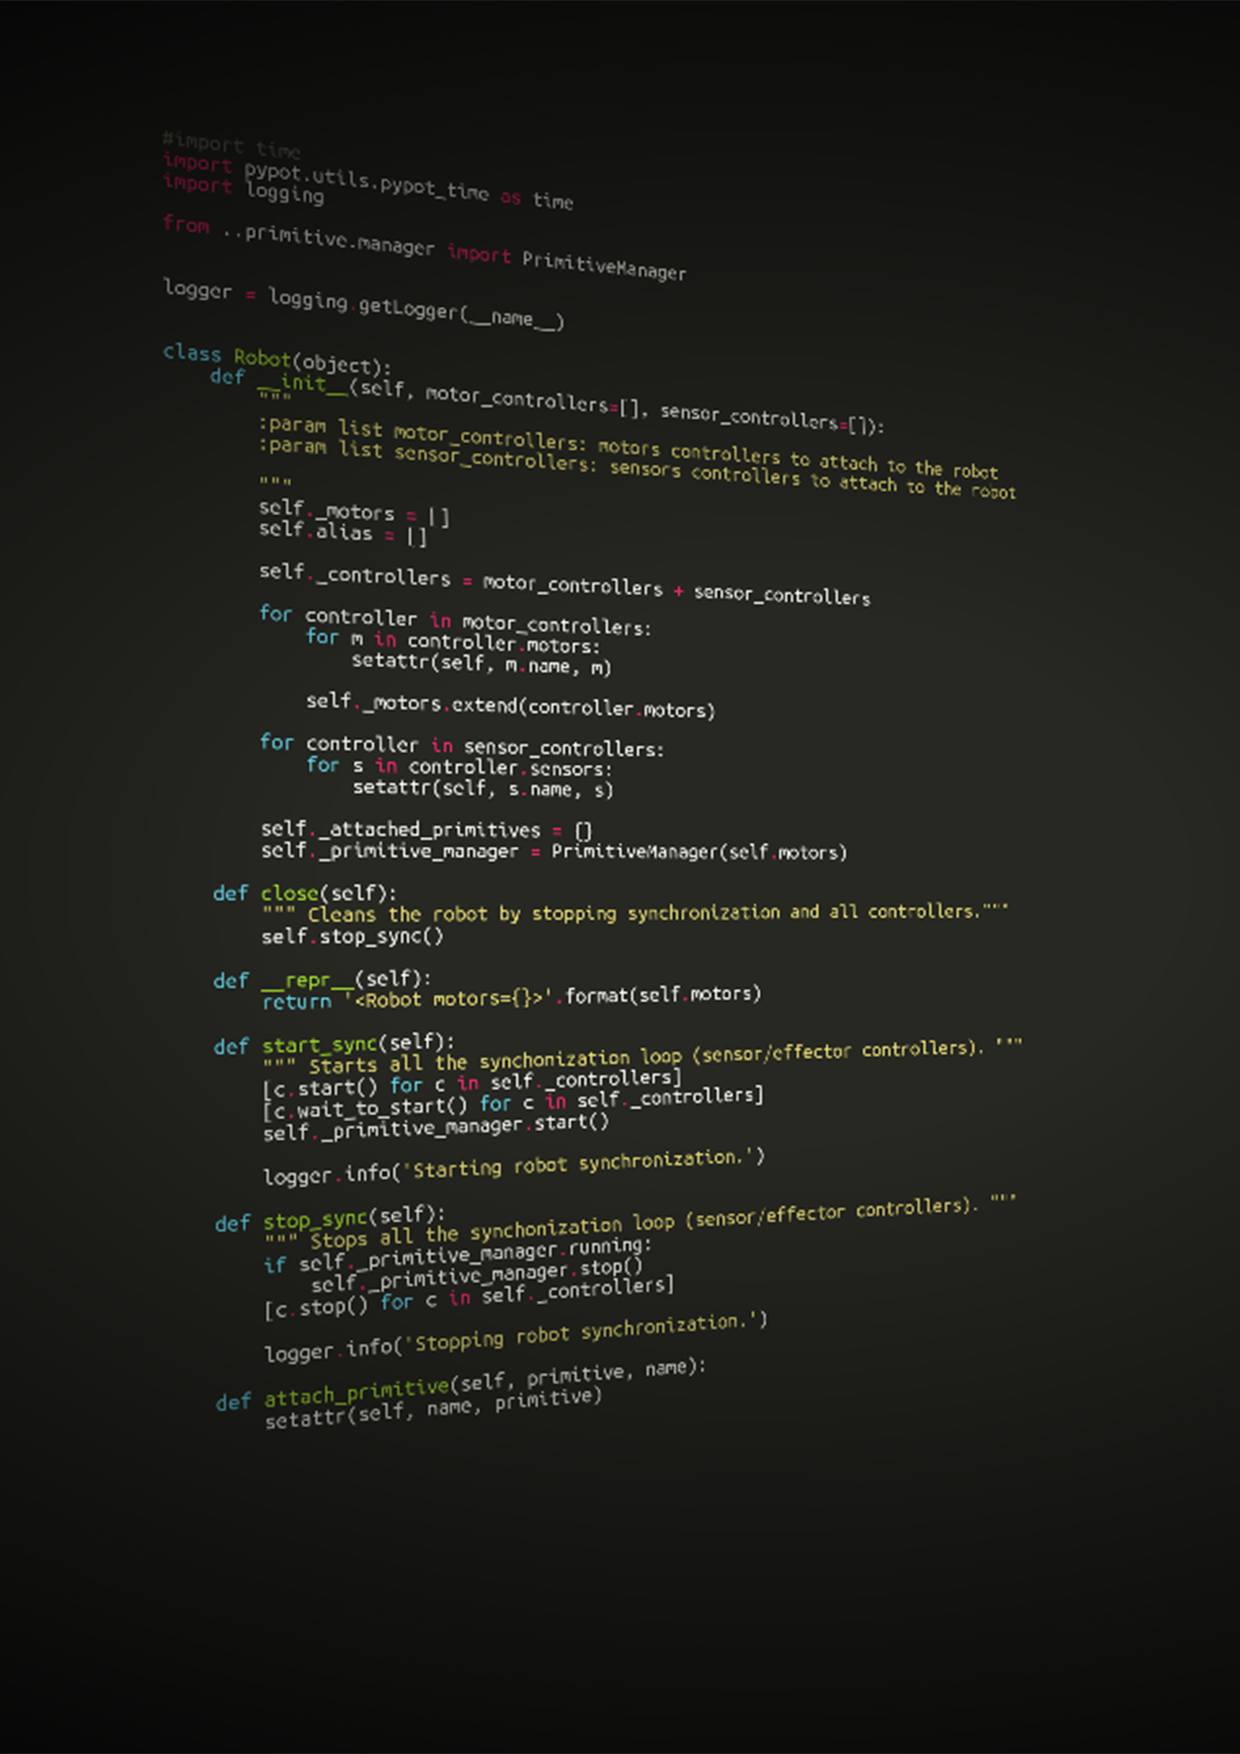
\includepdf{../media/chapter_illustration/pypot}
\chapter{Pypot: An open source modular python library for robot control} % (fold)

\section{Introduction} % (fold)

Poppy was designed to be a research platform for freely exploring morphological variations. Although Poppy meets "hardware" needs, control of the platform is of course crucial. Where more conventional robots have a fixed mechanical and sensorimotor morphology, having a platform that can be fully modified changes the low-level control architecture issues.
We decided to develop a new robotic library control. Called pypot (see \figurename~\ref{fig:pypot_logo}), this library mostly developed by Pierre Rouanet, is adapted to the challenges of morphological exploration and experimentation. Moreover, development begun early in the design of Poppy, and shares the same guidelines and objectives i.e. being robust, modular, versatile and easy to use.

\begin{Row}%
\begin{Cell}{2}

\begin{NFfigure}
    \begin{center}
        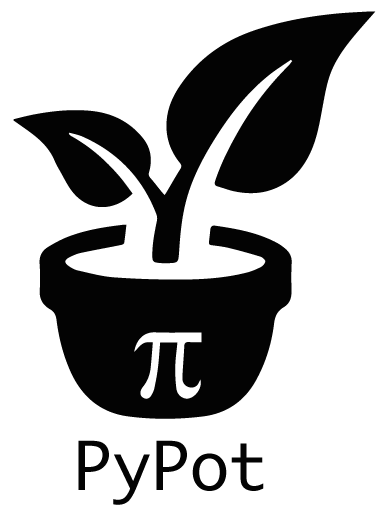
\includegraphics[width=0.8\linewidth]{PyPot_logo_black_transparentbg.png}
    \end{center}
    \caption{The pypot library logo}
    \label{fig:pypot_logo}
\end{NFfigure}

\end{Cell}
\begin{Cell}{4}
Toward these goals, pypot is a library written in Python and developed to make it easy and fast to control custom and modular robots. In particular, pypot has been designed with a simple and easy to use API, a fully modular and customizable architecture, and key-features adapted to the robotic experimentation issues.
\end{Cell}
\end{Row}





\section{Control of custom robot made simple with pypot} % (fold)

A main preoccupation during the development of pypot is the achievement of a very easy-to-use library for the end user. For this purpose, pypot has been entirely written in Python to allow for fast development, easy deployment (cross-platform) and quick scripting by non-necessary expert developers. In particular, the API is simple and permits to write complex behaviors with just few-line of code.

This is made possible with a layered architecture based on:

\begin{itemize}
    \item Fast and robust low-level API that directly encapsulates the communication protocol for setting and acessing hardware values.
    \item A controller which automatically ensures the update of sensorimotor values (get/set) at a predefined frequency. This method encapsulates the low-level API to prevent the writing repetitive request and optimize latency.
    \item Finally, a robot layer can generate automatically a whole robot API giving access of the whole sensorimotor space with just a few lines of code.
\end{itemize}

While low-level layers allow for modularity and customization, the high-level abstracts all the complexity into simple end user API. We will describe more in details how this architecture works in the next sections.

% Also, it benefits from the Python community with numpy/scipy and machine learning libraries such as scikit-learn.

\subsection{The Dynamixel controller} % (fold)

PyPot handles the low-level communication with dynamixel motors from Robotis. Using a USB communication device such as USB2Dynamixel or USB2AX, it opens serial communication with Robotis motors (MX, RX, AX) using communication protocols TTL or RS485. More specifically, it allows easy access (both reading and writing) to the different registers of any dynamixel motors\footnote{The whole list of registers can directly be found on the Robotis website: \url{http://support.robotis.com/en/product/dynamixel/mx_series/mx-28.htm\#Control_Table}}. Those registers includes values such as position, speed or torque.


While the Dynamixel Low-level IO provides access to all functionalities of the dynamixel motors, it forces to have synchronous calls which can take a non-negligible amount of time. In particular, most programs will need to have a really fast read/write synchronization loop, where we typically read all motor positions, speeds, loads and set new values, while in parallel we would like to have higher level code that computes those new values.

On top of the low-level, a Dynamixel controller can be added which defines synchronization loops that will read/write the registers of dynamixel motors at a predefined frequency automaticcaly run in background.
Whenever one of the values is accessed, it is actually the most recent versions that have been read at the frequency of the loop. Thus there is no need to wait the answer of a read command to access data (this can take some time) so that algorithms with heavy computation do not encounter a bottleneck when values from motors must be known. The attributes of those “software” motors are automatically synchronized with the real “hardware” motors.

The controller is actually a module (see section REF) and can be changed as the user needs. Yet by default pypot has a base controller which already defines synchronization loops, more exactly:

\begin{itemize}
    \item reads the present position, speed, load at 50Hz,
    \item writes the goal position, moving speed and torque limit at 50Hz,
    \item writes the pid or compliance margin/slope (depending on the type of motor) at 10Hz,
    \item reads the present temperature and voltage at 1Hz.
\end{itemize}



\subsection{Robot abstraction} % (fold)you

The robot abstraction allows, from a configuration, to generate both all controllers needed to control a whole robot. More precisely, through the use of the class Robot it is possible to:

\begin{itemize}
    \item automatically initialize all connections (make transparent the use of multiple USB2serial connections),
    \item define offset and direct attributes for motors,
    \item automatically define accessors for motors and their most frequently used registers (such as goal\_position, present\_speed, present\_load, PID, compliant),
    \item define read/write synchronization loop that will run in background.
\end{itemize}

The configuration, described as a Python dictionary\footnote{The configuration can be written in the Python script or can be loaded from any file that can be loaded as a dict (e.g. a JSON file).}, contains several important features that help build both the robot and the software to manage the robot. The important fields are listed below:

\begin{itemize}
    \item controllers - This key holds the information pertaining to a controller and all the items connected to its bus.
    \item motors - This is a description of all the custom setup values for each motor. Meta information, such as the motor access name or orientation, is also included here. It is also there that we can set the angle limits of the motor.
    \item motorgroups - This is used to define alias of a group of motors (e.g. left\_leg).
\end{itemize}

To give a complete overview of what a config can look like, the \codename~\ref{code:robot_config_file} is an example of the config dictionnary of a simple 6-DoF ergo-robot.

\lstinputlisting[
    language = XML,
    caption = {Creating a robot},
    label = {code:robot_config_file},
    float = p]
    {code/robot_configuration.json}


The robot abstraction encapulates multiple Dynamixel controller to read/write all the registers of a robot at a predefined frequency. The user only has to specify the configuration dictionnary of his robot using the from\_config() function. The robot configuration can also loaded/saved as a JSON format.

Here is an example of how to create a robot:
\begin{lstlisting}[language = Python]
import pypot.robot

# Load the configuration file
my_robot = pypot.robot.from_config('ergo_robot.json')

# Launch robot sensorimotor synchronization
my_robot = start_sync()
\end{lstlisting}


Then making the robot move is only one line of code:
\begin{lstlisting}[language = Python]
my_robot.base_tilt_lower.goal_position = 120
\end{lstlisting}

Yet the motor 'base\_tilt\_lower' will not reach the 120 degree position, but actually 90 degree because its config file (\codename~\ref{code:robot_config_file}) set the angle limit to [-90, 90].

Thus user can simply and safely uses the robot with just scripting the behavior he wants.



\subsection{Move recording} % (fold)
\label{sub:move_recording}

% subsection move_recording (end)


\section{Modular environment} % (fold)



\begin{figure}[p]
    \begin{center}
        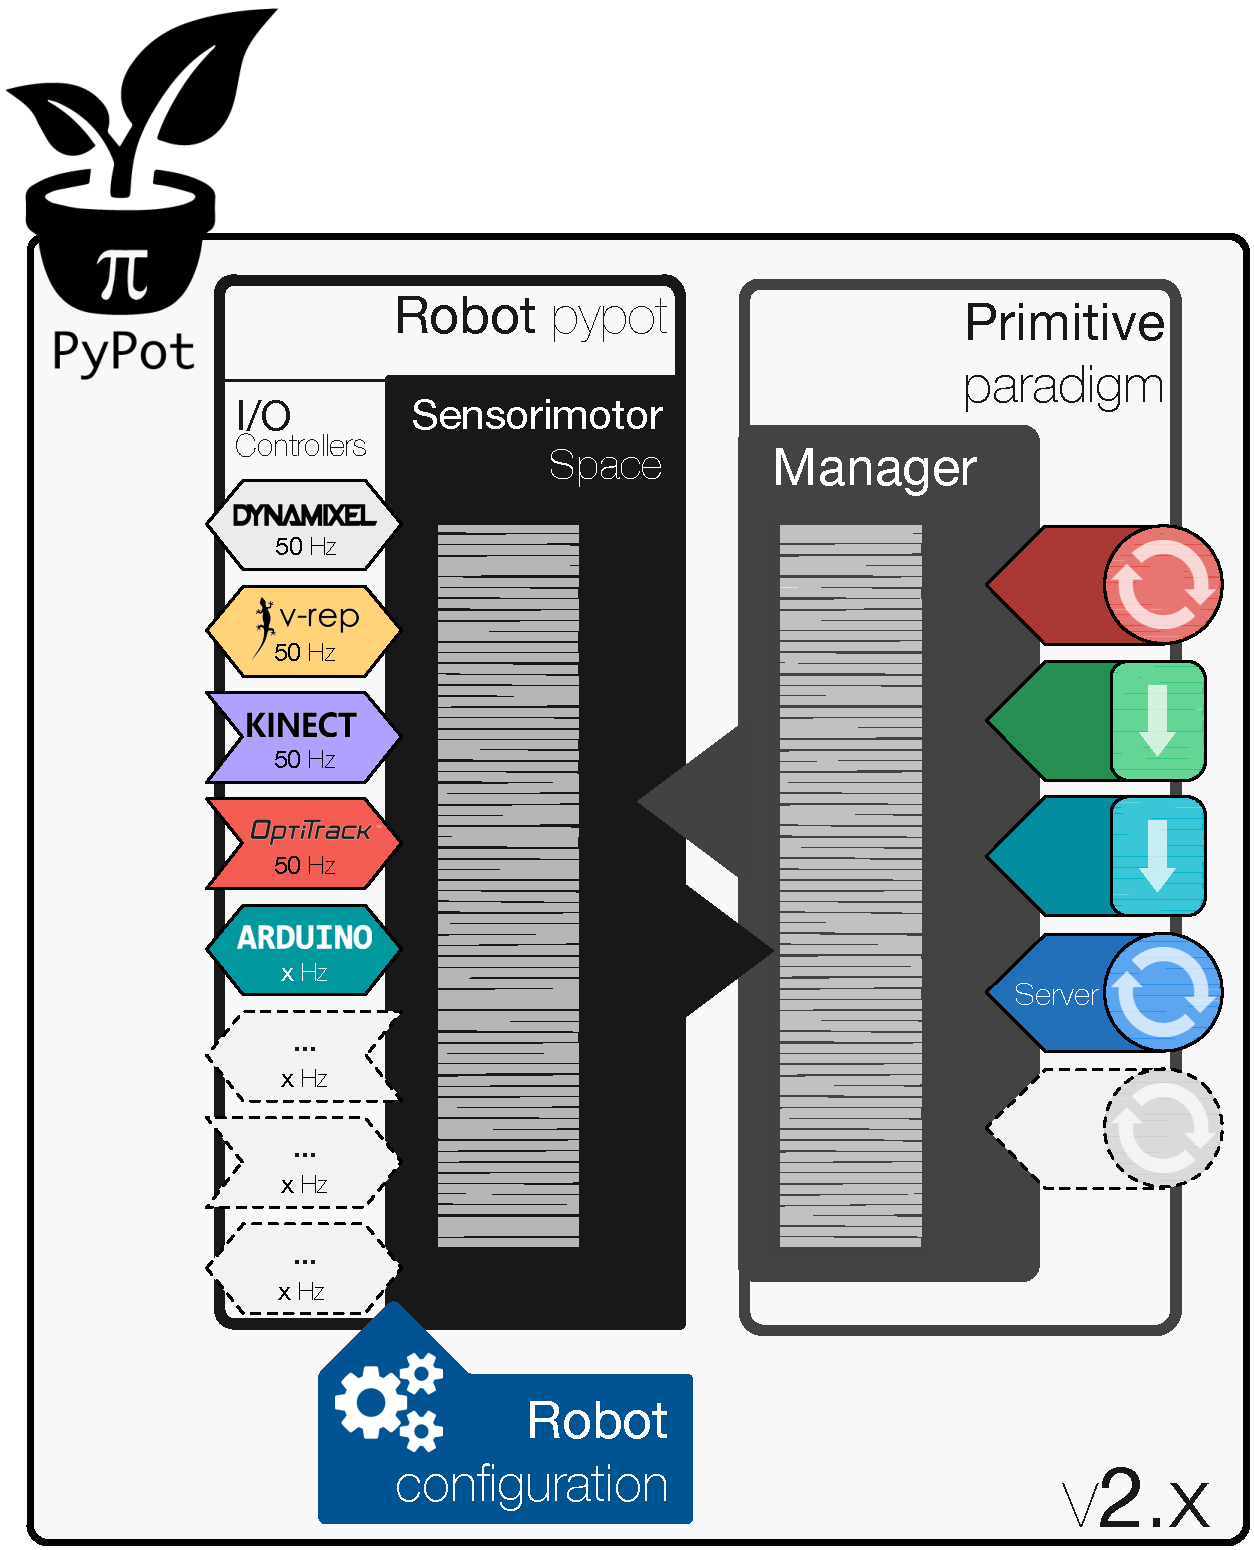
\includegraphics[width=\linewidth]{pypot.pdf}
    \end{center}
    \caption{Caption here}
    \label{fig:pypot-modular-architecture}
\end{figure}


\subsection{I/O controllers} % (fold)




\subsection{Primitive paradigms} % (fold)
We call Primitive any simple or complex behavior applied to a Robot. A primitive can access all sensors and effectors in the robot. A primitive is supposed to be independent\footnote{The independence of primitives is really important when one create complex behaviors - such as balance - where many primitives are needed. Adding another primitive - such as walking - should be direct and not force the rewrite of everything. Furthermore, the balance primitive could also be combined with another behavior - such as shoot a ball - without modifying it.} of other primitives. In particular, a primitive is not aware of the other primitives running on the robot at the same time. We imagine those primitives as elementary blocks that can be combined to create more complex blocks in a hierarchical manner.

To ensure this independence, the primitive is running in a sort of sandbox. More precisely, this means that the primitive has not direct access to the robot. It can only request commands (e.g. set a new goal position of a motor) to a PrimitiveManager which transmits them to the “real” robot. As multiple primitives can run on the robot at the same time, their request orders are combined by the manager\footnote{The primitives all share the same manager. In further versions, we would like to move from this linear combination of all primitives to a hierarchical structure and have different layer of managers.}.

The manager uses a filter function to combine all orders sent by primitives. By default, this filter function is a simple mean but you can choose your own specific filter (e.g. add function).

To write a primitive, the user only needs to create a subclass of the Primitive class. It provides basic mechanisms (e.g. connection to the manager, setup of the thread) to allow the direct “plug” of novel primitives to a robot and run it.

Currently there are two kind of primitives.


\lstinputlisting[
    language = Python,
    caption = {Creating a robot},
    label = {code:primitive},
    float,
    floatplacement = h]
    {code/primitive.py}

\lstinputlisting[
    language = Python,
    caption = {Creating a robot},
    label = {code:loop_primitive},
    float,
    floatplacement = h]
    {code/loop_primitive.py}

The primitive can be start(), stop(), pause() and resume(). Unlike regular python thread, primitive can be restart by calling again the start() method.

When overriding the Primitive, you are responsible for correctly handling those events. For instance, the stop method will only trigger the should stop event that you should watch in your run loop and break it when the event is set. In particular, you should check the should\_stop() and should\_pause() in your run loop. You can also use the wait\_to\_stop() and wait\_to\_resume() to wait until the commands have really been executed.


\lstinputlisting[
    language = Python,
    caption = {Creating a robot},
    label = {code:start_primitive},
    float,
    floatplacement = h]
    {code/start_primitive.py}

\lstinputlisting[
    language = Python,
    caption = {Creating a robot},
    label = {code:attach_primitive},
    float,
    floatplacement = h]
    {code/attach_primitive.py}





\subsection{Switch between simulator and real world} % (fold)

As it is often easier to work in simulation rather than with the real robot, Pypot has been linked with the V-REP simulator\footnote{\url{http://www.coppeliarobotics.com/features.html}}. It is described as the “Swiss army knife among robot simulators” and is indeed a very powerful tool to quickly (re)create robotics setup. Moreover, we chose to integrate this particular simulator first because it shares distinctive features with the Poppy project, i.e being cross-platform, easy-to-use, extensible and open source\footnote{Actually V-REP has a double license Commercial/GPL so either one pay and can keep his customizations or have to release all modification under GPL.}

\begin{figure}[tb]
    \begin{center}
        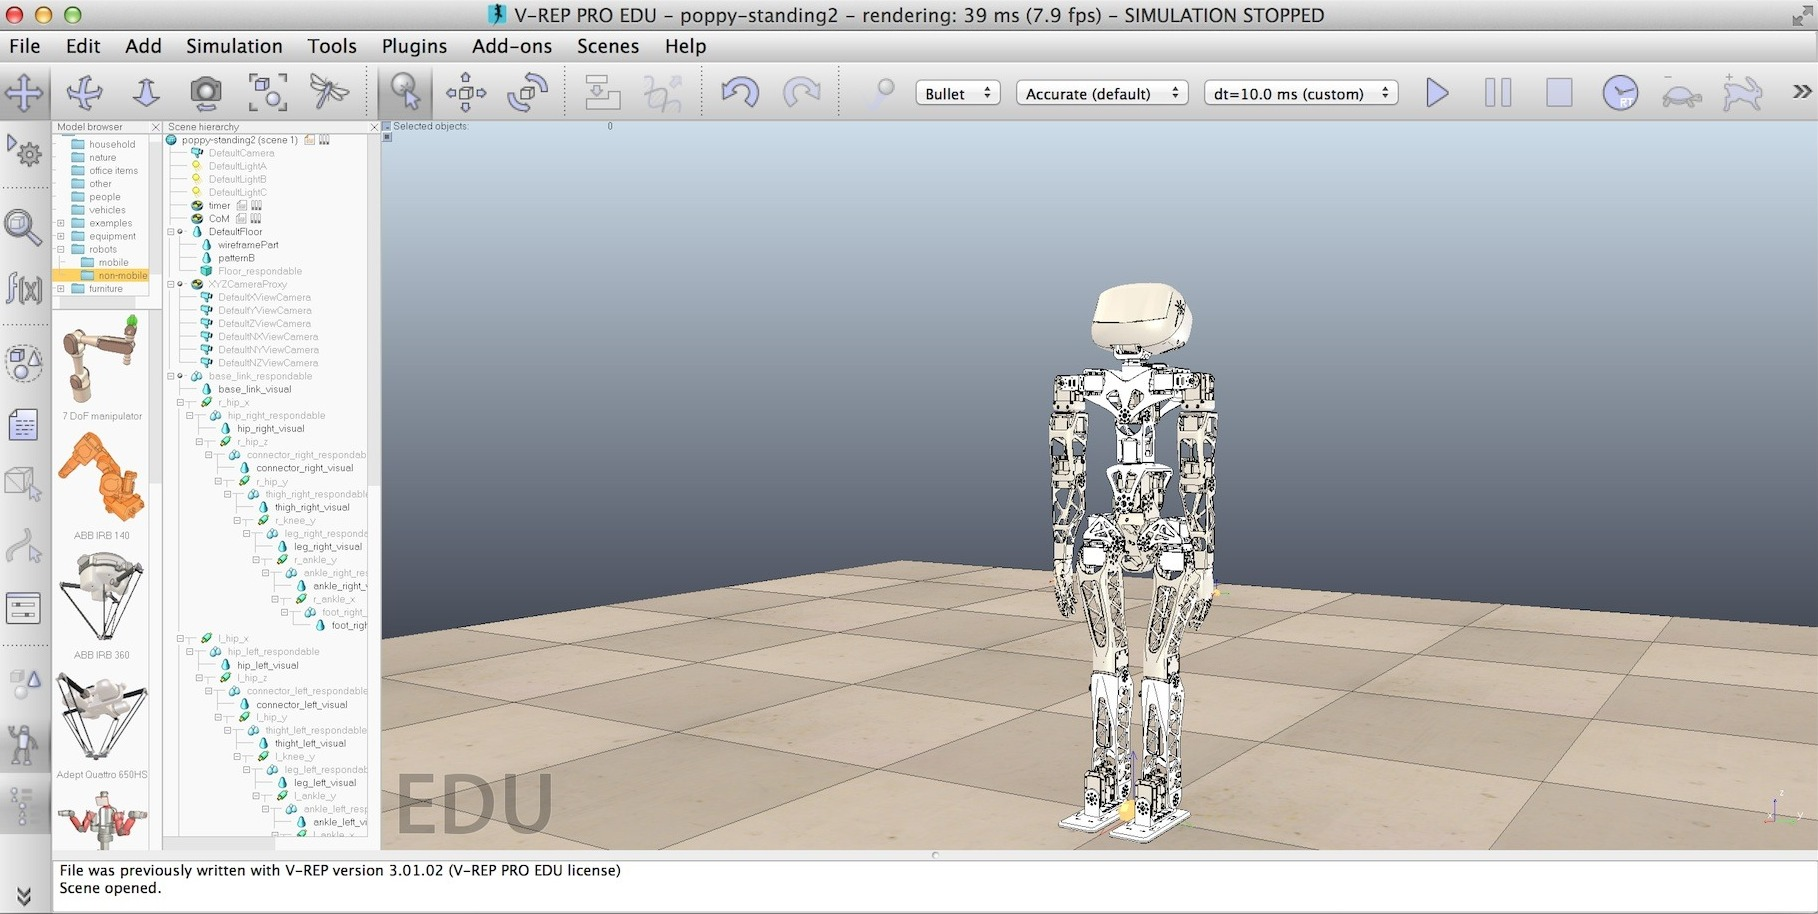
\includegraphics[width=\linewidth]{pypot_vrep.jpg}
    \end{center}
    \caption{Caption here}
    \label{fig:pypot-vrep}
\end{figure}


The connection with V-REP was created using the I/O controllers presented previously and the V-REP’s remote API.
Thanks to the low-level modularity of pypot, it permits to seamlessly switch from your real robot to the simulated one because it only require to switch the low-level I/O controller from the Dynamixel (DxlIO class) one to the V-REP one (VrepIO class).

The switch between the simulation and the real robot is possible with a single line of code, and in most case, only requires to change the way the robot is instantiated see \codename~\ref{code:vrep_pypot_switch}.

\lstinputlisting[
    language = Python,
    caption = {Creating a robot},
    label = {code:vrep_pypot_switch},
    float = h]
    {code/vrep_pypot_switch.py}

In addition, it provides some extended feature relative to the need we have in a robot simulator, among them:
load a scene, start/stop/restart a simulation, pause/resume the simulation, get an object position/orientation.
Yet not all dynamixel registers have their V-REP equivalent. For the moment, only the control of the position is used but it will be completed in the future. Also more advanced features can be easily added thanks to the controller abstraction.

The controller was done for V-REP but the same work could be done with any other simulator and the switch should be as straightforward.


\subsection{Extensible API} % (fold)

We added the possibility to remotely access and control your robot through TCP network. This can be useful both to work with client/server architecture (e.g. to separate the low-level control running on an embedded computer and higher-level computation on a more powerful computer) and to allow you to plug your existing code written in another language to the PyPot’s API.

We defined a protocol which permits the access of all the robot variables and method (including motors and primitives) via a JSON request. The protocol is entirely described in the section Protocol below. Two transport methods have been developed so far:

\subsubsection{HTTP server} % (fold)

The HTTPServer is based on the bottle python framework (http://bottlepy.org/). We have developed a sort of REST API based on the protocol described above:

\begin{itemize}
    \item GET /motor/list.json
    \item GET /primitive/list.json
    \item GET /motor/<name>/register.json (or GET /<name>/register.json)
    \item GET /motor/<name>/<register> (or GET /<name>/<register>)
    \item POST /motor/<name>/<register> (or POST /<name>/<register>)
    \item POST /primitive/<prim\_name>/call/<meth\_name> (or GET /<prim\_name>/call/<meth\_name>)
    \item POST /request.json
\end{itemize}


\lstinputlisting[
    language = Python,
    caption = {Creating a robot},
    label = {code:http_server},
    float,
    floatplacement = h]
    {code/http_server.py}


\subsubsection{ZMQ server} % (fold)

The Zmq Server used a Zmq socket to send (resp. receive) JSON request (JSON answer). It is based on the REQ/REP pattern. So you should always alternate sending and receiving. It will probably be switched to PUB/SUB soon.

Zmq has been chosen as it has been binded to most language\footnote{\url{http://zeromq.org/bindings:_start}} and can thus be used to connect code from other language to PyPot. For instance, we used it to connect RLPark\footnote{RLPark is a Java reinforcement learning library developed by Thomas Degris to experiment with online learning algorithms on robots and benchmarks, see \url{http://rlpark.github.io/}} to PyPot.

The zmq server is faster than the HTTP version and should be preferred when working with high frequency control loops.

\lstinputlisting[
    language = Python,
    caption = {Creating a robot},
    label = {code:zmq_server},
    float,
    floatplacement = h]
    {code/zmq_server.py}


In particular, whose extension could be use to create a monitor interface using web technology.






\section{Limits} % (fold)


\subsection{Performance} % (fold)

\subsection{The primitive architecture: The Good, the Bad and the Ugly} % (fold)
The high level design allows the use of primitives.
Primitives are ...
This features is really powerful has it allows to create complex behavior as a sum of simple behavior.
However the interaction between them is tricky and can lead to undesired behavior.


\lstinputlisting[
    language = Python,
    caption = {Creating a robot},
    label = {code:mockup_motor},
    float,
    floatplacement = h]
    {code/mockup.py}




\section{Conclusion} % (fold)


\subsection{Documented} % (fold)


\section{Discussion} % (fold)

\subsection{Why not using ROS instead ?} % (fold)

A famous robotics software is the Robot Operating System\footnote{The Robot Operating System (ROS) is a flexible framework for writing robot software. It is a collection of tools, libraries, and conventions that aim to simplify the task of creating complex and robust robot behavior across a wide variety of robotic platforms.}. ROS is very widespread in the research community and one could quite rightly question the choice we made to create a whole new architecture rather than using well known and efficient one.

Actually ROS has several aspects not fitting with the objectives we have. Indeed, using ROS is not a simple task. The installation is only recommended on one precise Ubuntu distribution\footnote{ROS Hydro only supports Precise, Quantal, and Raring for debian packages \url{http://wiki.ros.org/indigo/Installation}}, and the whole architecture is of course powerful but difficult to set and maintain. Also changing the low-level is complex and requires hacks, sometimes not really elegant. Finally, ROS require high computational power, which make it difficult to embed on small computer.

In the Poppy project, we are trying to create a multidisciplinary robotic community, involving as a result, non-robotics experts. Thus, we endeavor to pull down the complexity of using Poppy. Toward this goal, we need a simple user interface/API and a lightweight library easy to setup whichever system used. Finally, ROS is very modular for high-level but we desire to have a modular low-level control.

For all the above mentioned reasons we considered it should be more simple and effective to create a novel lightweight robot control library than adapting ROS to our needs.
